\section{Process' Perspective}

\subsection{Developer interactions}
Throughout the development of the project, the team has interacted primarily through Discord. Further, the team met physically on Tuesdays.

\subsection{Team organization}
We organized ourselves as a cross-functional team. Sometimes we worked on tasks individually but for the majority of the project we worked together, 
typically in pairs. Every opinion and input from each team member was acknowledged equally. 

\subsection{CI/CD chains}
Our CI/CD chain consists of the following GitHub Actions workflows:
\begin{itemize}
    \item Continuous-deployment - Builds Docker image, pushes it to the registry, SSH onto the server, and runs the deployment script.
    \item Dev - Functions as the Continuous-deployment workflow but deploys to a test environment similar to production.
    \item Test - Runs the test Docker compose file which creates a closed environment with the code on the current branch and runs the test.
    \item Main Release - This uses an external action namely \textit{rymndhng/release-on-push-action@master} for creating a release every time a push to main is made.
    \item Lint - Uses the external action 'golangci/golangci-lint-action@v3' which checks the code with multiple linters.
\end{itemize}

Every time a pull request was made to a branch, the 'Lint' and 'Test' workflows were run. The workflows that handled deployment were triggered manually.
Further, we have set up CodeClimate and SonarCloud to help us maintain an appropriate code standard. The SonarCloud check runs on every pull request targeting our main branch (see section \ref{branching} for a description of the 
branching structure).

\subsection{Organization of Repository}
The project only consists of a single repository containing the application. We chose this because it is a small application and thus splitting it into multiple
repositories would have complicated the development process unnecessarily. This single repository contains several folders:

\renewcommand{\arraystretch}{3}
\begin{table}[H]
    \centering
    \resizebox{\textwidth}{!}{%
    \begin{tabular}{|l|l|}
    \hline
    \Large\textbf{.github/workflows} & \Large Contains all our workflow files used with GitHub Actions.                                                                                                          \\ \hline
    \Large\textbf{api\_test}         & \Large Includes files to run the simulator and a test of the API. Primarily used during the development of the endpoints.                                                     \\ \hline
    \Large\textbf{remote\_files}     & \Large Has all files that are used when deploying to the server. This includes various logging and monitoring files, \\ & \Large our deploy script, and the docker-compose file.      \\ \hline
    \Large\textbf{report}            & \Large This folder is where our report files are saved.                                                                                                                   \\ \hline
    \Large\textbf{src}               & \Large Contains all our application code which is further divided into subfolders, thereby separating the logic \\ & \Large of the system.                                            \\ \hline
    \Large\textbf{tests}             & \Large Our test files are located in this folder. It contains a Docker file, a docker-compose file, and a test file to \\ &  \Large run our tests without external impact. \\ \hline
    \end{tabular}%
    }
    \caption{Repository folders}
    \label{tab:repo_folders}
    \end{table}

\subsection{Branching strategy} \label{branching}
We used two static branches (main and dev) as part of our branching strategy throughout the development of the project. 
The main branch was only used for functioning and tested code, and was deployed to production. The dev branch was used for development and testing. Additional branches were created when new functionality was to be implemented, or bugs had to be
fixed. All temporary branches were derived from the main branch. An example of our general branching strategy can be seen in figure \ref{fig:gen_branch} and \ref{fig:ex_branch}.

\begin{figure}[H]
    \centering
    \captionsetup{justification=centering,margin=1cm}
    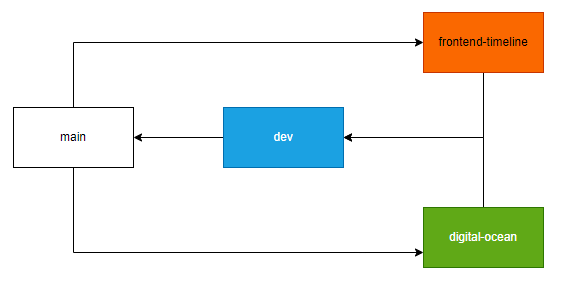
\includegraphics[width=0.7\linewidth]{report/images/branching.png}
    \caption{General branching strategy}
    \label{fig:gen_branch}
\end{figure}

\begin{figure}[H]
    \centering
    \captionsetup{justification=centering,margin=1cm}
    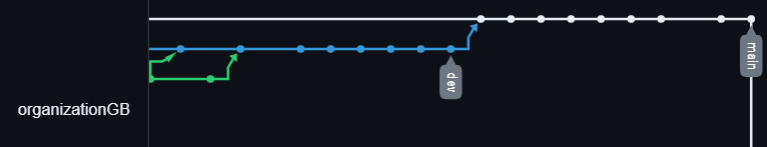
\includegraphics[width=0.7\linewidth]{report/images/git_branching.png}
    \caption{Example use of branching strategy}
    \label{fig:ex_branch}
\end{figure}

It can be seen that the temporary branches are derived from the main branch, and when the functionality is implemented, 
it is merged into the dev branch to be tested before the code is put into production. 

\subsection{Development process and tools}
When meeting on Tuesdays we discussed what needed to be done if we weren't already working on a task. We tried to start using a Kanban board but due to us not establishing 
clear guidelines on how to use the tool, we didn't manage to successfully implement it. In our development process, we utilized pair programming a lot. This also lead to an iterative development process in that we pushed small changes often to switch programmer. Further, the team agreed that when larger new implementations were to be introduced to the main or dev branch, a pull request should be made to allow team members to review the code.

\subsection{Monitoring}
The deployed MiniTwit application was monitored using Grafana, which is a dashboard web application for visualization of data. 
We used Grafana to monitor the simulator's interaction with our application. On our dashboard, we included a visualization of the CPU load percentage as well as an overview of the duration of requests to the different endpoints. Here it was possible to see the metrics for a single endpoint. This allowed us to analyze CPU load spikes, as they might be due to resource-intensive endpoint requests. Additionally, we monitored the total number of responses to assess the availability of the application. \\

Data was collected for visualization; we used Prometheus, an open-source monitoring system that collects and stores various metrics data from the web server. Prometheus pulls the metric data from the MiniTwit application from a metrics endpoint and stores it so it can be queried by Grafana and shown in the dashboard.

\subsection{Logging}
Our logging setup is based on Elasticsearch, Kibana, and Filebeat as visualized by figure \ref{fig:logging}. These open-source tools are all developed by the same company which eases the integration process. Filebeat collects logs from the application containers after which they are forwarded to Elasticsearch. 
Elasticsearch is a search and analytics engine and here the logs are indexed so they can be queried by Kibana where the logs can be visualized by interactive dashboards.  
In our setup, Filebeat appends the container name to all logs so they can be filtered and visualized per-container basis.

\begin{figure}[H]
    \centering
    \captionsetup{justification=centering,margin=1cm}
    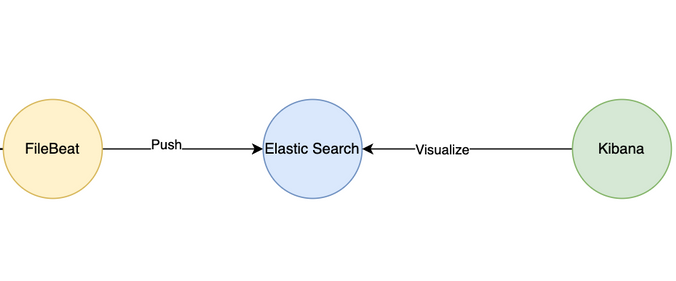
\includegraphics[width=0.8\linewidth]{report/images/logging.png}
    \caption{Logging setup}
    \label{fig:logging}
\end{figure}

\subsection{Security assessment}
From our security assessment, we learned that we were most at risk of attacks based on unauthorized access to our codebase and our weak authentication and authorization mechanisms. The first risk was likely to occur as it was possible to find passwords and usernames for the database in our public codebase. We made sure that these were no longer stored directly in the source code by importing them from GitHub secrets instead. The second identified risk could be improved by changing the default passwords to follow security standards.  

\subsection{Scaling and load balancing}

Our choice for scaling strategy was to divide our services into micro-services and deploy them in a Docker Swarm cluster. This meant that we could scale horizontally and vertically. In this design, we had multiple instances of loadbalancers, that would be placed on different nodes. The purpose of having multiple instances of the MiniTwit application services is that we try to ensure up-time if a container on another server node breaks for some unforeseen reason. Our services that were single-points of failure given the design, were Redis, Postgres, and Elasticsearch, the latter only meaning our logging would be down. 

Since we used Docker Swarm to orchestrate our micro-services, we would now be able to take advantage of their built-in functions in the update strategy. Our choice was to use a stop-first rolling update strategy, which is mentioned in the Docker Swarm documentation \footnote{https://docs.docker.com/engine/swarm/swarm-tutorial/rolling-update/}. This aims to achieve a close to zero downtime as we roll out updates for the application containers and allows us to gracefully update each container as we move to a newer version of the application.

\subsection{AI-assistants}
The team has used AI-assistants to aid in the development and deployment of the MiniTwit application. We used OpenAI's ChatGPT and Phind.

Using these assistants aided us because they provided a quick overview of the possibilities with short and general explanations regarding the technologies we used as well as how to approach development tasks, such as describing the different components used in a docker-compose file or bootstrapping a Go application using the Gin framework. However, using them also hindered us as we often had to double-check whether the information provided was accurate and ended up using more time than if we obtained the information without them. 

%%Bootstrap = to get one going/started